\documentclass{report}
\usepackage{pdfpages}
\usepackage{graphicx} 
\usepackage{dirtytalk}
% \usepackage{arydshln}
\usepackage{lmodern}
\usepackage{booktabs}
\usepackage{listings}
\usepackage{float}
\usepackage{siunitx}
\usepackage{amsmath}
\usepackage{rotating}
\usepackage{arydshln}
\usepackage[hidelinks]{hyperref}
\usepackage[ngerman]{babel}
\usepackage[a4paper, total={6in, 8in}]{geometry}
\begin{document}

\includepdf[pages=-]{./PDFs/Deckblatt_P1}
\begin{titlepage}
    \begin{center}
        \vspace*{1cm}
            
        \Huge
        \textbf{Auswertung und Protokoll}
            
        \vspace{0.5cm}
        \LARGE
        Zum Versuch AKU - Akustik im Haushalt

        \vspace{1.8cm}

        \textbf{Jonas Müther}
        \vfill
            
        P1 Praktikum\\
       
            
        \vspace{0.8cm}
  

        \vspace{1.8cm}
        \Large
        LMU München \\
        Physik B.Sc.\\
        Deutschland\\
        2026
            
    \end{center}
\end{titlepage}
\tableofcontents

\newpage
\chapter{Vorbereitung}

\section{Versuchsvorbereitung und Grundlagen des Versuchs}
\subsection{Theoretischer Hintergrund}
\subsubsection{Wellen \& Wellenausbreitung}
\begin{list}{$\bullet$}{}
    \item Modell: Einzelne Masseelemente, die elastisch miteinander gekoppelt sind und harmonisch schwingen
    \item Auslenkung eines Massenelemts wird durch Kopplung an das nächste weitergegeben, dieses schwingt aufgrund der Trägheit zeitlich verzögert
    \item das angeregte Massenelemt gibt die Schwingung wiederrum weiter, usw.
    \item Es entsteht eine Sinusförmige Kurve, auf der die Massen zu einem festen Zeitpunkt liegen
\end{list}
\subsubsection{Charakteristische Größen}
\begin{list}{$\bullet$}{}
    \item Wellenlänge $\lambda$: Abstand von einem Massenelement zum nächsten, das sich im selben Schwingungszustand befindet
    \item Phasengeschwindigkeit $v$: Geschwindigkeit der Bewegung eines Schwingungszustands im Medium
    \item   \begin{equation}
                v = \frac{\lambda}{T} = f\lambda
            \end{equation}
    \item Je größer die Köpplung und je kleiner die Masse, desto größer wird die Phasengeschwindigkeit
    \item   \begin{equation}
                v = \sqrt{\frac{E}{\rho}}
            \end{equation}
    \item Die Schallgeschwindigkeit ist Temperaturabhängig:
    \item   \begin{equation}
                v = \sqrt{\gamma \frac{RT}{M}}
            \end{equation}
\end{list}
\subsection{Stehende Wellen}
\begin{list}{$\bullet$}{}
    \item Entsteht durch Überlagerung von gegenläufigen Wellen mit gleicher Wellenlänge, Amplitude und Geschwindigkeit
    \item Oszillatoren schwingen Permanent, aber Welle als ganzes bewegt sich nicht
    \item Knoten (Punkte mit dauerhafre Amplitude von 0) und Bäuche (Punkte bei maximaler Schwingungsamplitude)
    \item Abstand zwischen zwei Knoten: $d=\frac{\lambda}{2}$
\end{list}
\begin{figure}[H]
    \centering
    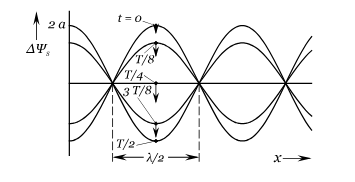
\includegraphics[width=.5\textwidth]{./Images/Stehende Welle.png}
    \caption{Stehende Welle}
    \label{fig:StWelle}
\end{figure}
\subsection{Oberschwingungen}
\begin{list}{$\bullet$}{}
    \item Anregung einer Schwingung in einem Rohr nur mit bestimmte diskrete Frequenzen
    \item Nur die stehenden Wellen, die die Randbedingungen erfüllen können (Knoten am geschlossenen Ende und Bauch am offenen Ende)
    \item Einseitig offenes Rohr: 
    \begin{equation}
        \begin{split}
            f_n = \frac{v}{4L} (2n+1)
        \end{split}
    \end{equation}
\end{list}
\subsection{Helmholtz Resonator}
\begin{list}{$\bullet$}{}
    \item Aus dem Haushalt bekanntes Beispiel: Flasche
    \item Durch Pusten über das obere Ende der Flasche kommt es zur Schwingung des Luftvolumens im Flaschenhals (Luftkorken)
    \item Das eingeschlossene Volumen im Flaschenbauch wirkt wie eine Feder
    \item Die Federkonstante liegt bei 
        \begin{equation}
            \begin{split}
                k = \frac{\rho_o A^2 v^2}{V_0}
            \end{split}
        \end{equation}
    \item Effektiv schwingendes Volumen etwas größer als eingeschlossenes Volumen im Hals 
        \begin{equation}
            \begin{split}
                L_{eff} = L + \frac{cD}{2}
            \end{split}
        \end{equation}
        mit $c = 1.4621$ und $D$ Durchmesser des Flaschenhalses
    \item Resonanzfrequenz:
        \begin{equation}
            f = \frac{v}{2\pi}\sqrt{\frac{A}{V_0 L_{eff}}}
            \label{eq:HelmholtzResFreq}
        \end{equation}
\end{list}


\subsection{Versuchsdurchführung}
\subsubsection{TVI: Bestimmung der Schallgeschwindigkeit mithilfe eines Helmholtz Resonators}
In TV I wird die Schallgeschwindigkeit mithilfe eines Helmholtz Resonators bestimmt. Dazu werden zwei Flaschen verwendet. Eine Flasche geht vom Hals schnell in den Bauch über, die andere kontinuierlich.
Zunächst werden jeweils die geometrischen Eigenschaften der Flaschen bestimmt, dann werden die Resonanzfrequenzen für verschiedene Wasserfüllstände bestimmt $\Leftrightarrow$ unterschiedliche Volumina des Flaschenbauchs.
Der Wasserfüllstand sowie das Gesamtvolumen der Flasche wird durch eine Messung der Masse des Wassers in der Flasche bestimmt. Die Frequenzmessung geschieht mithilfe der App PhyPhox. 


\subsubsection{TVII: Grund- und Oberschwingungen im Kundtschen Rohr}
Ein beidseitig offenes Rohr aus Pappe (Verpackung für Leuchtarmbänder) wird im Raum fixiert. Ein Smartphone generiert mit der Phyphox App auf der einen Seite des Rohrs weißes Rauschen. Das andere
nimmt auf der anderen Seite ebenfalls mit der PhyPhox App das angeregte Frequenzspektrum auf. Zusätzlich wird eine Messung des Frequenzspektrums ohne Rohr zwischen den Smartphones durchgeführt.
Mit dieser sollen dann später Peaks herausgefiltet werden, die eventuell bereits ohne Rohr im weißen Rauschen vorhanden sind.


\newpage
\section{Versuchsprotokoll}
\subsection{Bilder der Versuchsaufbauten}

\subsection{Aufschrieb}
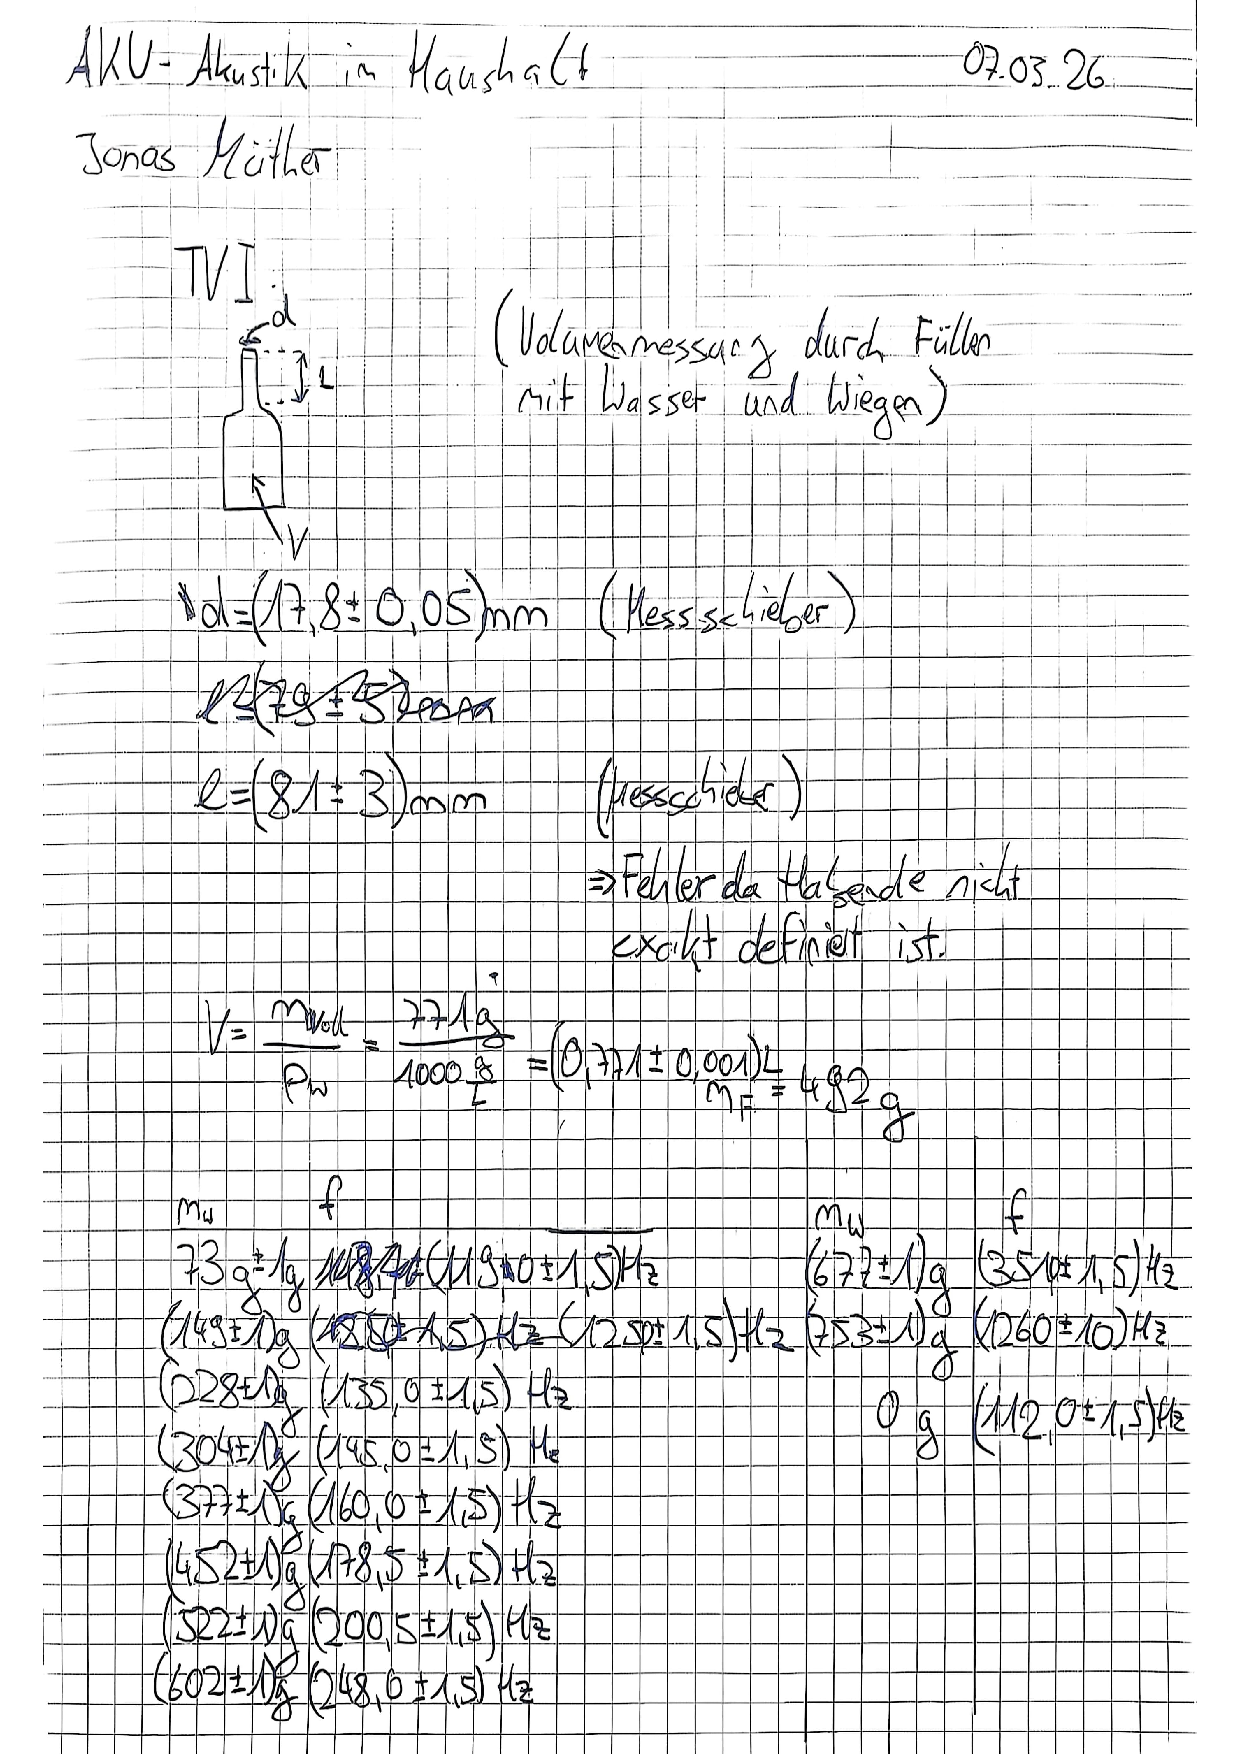
\includepdf[pages=-]{./PDFs/AKU_Durchfuehrung.pdf}

\newpage
\chapter{Auswertung}
\section{Teilversuch I: Helmholtz Resonator}
\subsection{Gemessene Daten}
In TVI wurden die Resonanzfrequenzen einer Flasche als Helmholtz Resonator bestimmt. Um damit die Schallgeschwindigkeit zu bestimmen wurde diese Frequenz für verschiedene
Füllstände bestimmt, was äquivalent zu einer Veränderung des effektiven Flaschenvolumens ist.
\subsubsection{Messwerte für Flasche 1}
Für eine Flasche mit raschem Übergang vom zylinderförmigen Flaschenhals in den Flaschenbauch wurden die Messwerte aus Tabelle \ref{tab:HelmholtzFreq} bestimmt.
\begin{table}[H]
    \centering
    \caption{Resonanzfrequenz von Flasche I für verschiedene effektive Volumina}
    \label{tab:HelmholtzFreq}
    \begin{tabular}{c c c}
        \hline
        $m_w (kg)$ &  $V_{eff}(\si{\ml})$ & $f_0(\si{\ml})$ \\
        \hline
        $0.000 \pm 0.001$ & $0.771 \pm 0.001$ &  $112.0 \pm 1.5$\\
        $0.073 \pm 0.001$ & $0.698 \pm 0.001$ &  $119.0 \pm 1.5$\\
        $0.149 \pm 0.001$ & $0.622 \pm 0.001$ &  $125.0 \pm 1.5$\\
        $0.228 \pm 0.001$ & $0.543 \pm 0.001$ &  $135.0 \pm 1.5$\\
        $0.304 \pm 0.001$ & $0.467 \pm 0.001$ &  $145.0 \pm 1.5$\\
        $0.377 \pm 0.001$ & $0.394 \pm 0.001$ &  $160.0 \pm 1.5$\\
        $0.452 \pm 0.001$ & $0.319 \pm 0.001$ &  $178.5 \pm 1.5$\\
        $0.522 \pm 0.001$ & $0.249 \pm 0.001$ &  $200.5 \pm 1.5$\\
        $0.602 \pm 0.001$ & $0.169 \pm 0.001$ &  $248.0 \pm 1.5$\\
        $0.677 \pm 0.001$ & $0.094 \pm 0.001$ &  $351.0 \pm 1.5$\\
        $0.753 \pm 0.001$ & $0.018 \pm 0.001$ &  $1260.0 \pm 10$\\
        \hline
    \end{tabular}
\end{table}
Außerdem wurden die folgenden geometrischen Abmessungen für die Flasche bestimmt:
\begin{equation}
    \begin{split}
        d &= 0.0178 \pm 0.00005 m \\
        l &= 0.081 \pm 0.003 m
    \end{split}
\end{equation}
\subsubsection{Messwerte für Flasche 2}
Für die Flasche mit langsamem Übergang vom Flaschenhals in den Flaschenbauch ergaben sich die Messwerte, die in Tabelle \ref{tab:HelmholtzFreq2} dargestellts sind. 
\begin{table}[H]
    \centering
    \caption{Resonanzfrequenz von Flasche II für verschiedene effektive Volumina}
    \label{tab:HelmholtzFreq2}
    \begin{tabular}{c c c}
        \hline
        $m_w (kg)$ &  $V_{eff}(\si{\ml})$ & $f_0(\si{\ml})$ \\
        \hline
        $0.000 \pm 0.001$ & $0.517 \pm 0.001$ &  $155.0 \pm 1.5$\\
        $0.049 \pm 0.001$ & $0.468 \pm 0.001$ &  $161.5 \pm 1.5$\\
        $0.101 \pm 0.001$ & $0.416 \pm 0.001$ &  $171.0 \pm 1.5$\\
        $0.151 \pm 0.001$ & $0.366 \pm 0.001$ &  $183.0 \pm 1.5$\\
        $0.198 \pm 0.001$ & $0.319 \pm 0.001$ &  $195.0 \pm 1.5$\\
        $0.254 \pm 0.001$ & $0.263 \pm 0.001$ &  $217.0 \pm 1.5$\\
        $0.299 \pm 0.001$ & $0.218 \pm 0.001$ &  $240.5 \pm 1.5$\\
        $0.355 \pm 0.001$ & $0.162 \pm 0.001$ &  $276.5 \pm 1.5$\\
        $0.403 \pm 0.001$ & $0.114 \pm 0.001$ &  $339.5 \pm 1.5$\\
        $0.454 \pm 0.001$ & $0.063 \pm 0.001$ &  $463.0 \pm 3$\\
        \hline
    \end{tabular}
\end{table}
Hier wurden folgende geometrische Abmessungen bestimmt:
\begin{equation}
    \begin{split}
        d &= 0.1703 \pm 0.0005 m \\
        l &= 0.130 \pm 0.005 m
    \end{split}
\end{equation}
\textit{Anmerkung: Die Länge des Flaschenhalses wurde bis zu dem Punkt der Flasche gemessen, an dem diese vollständig Zylinderförmig wird. Dieser Wert spielt allerdings
für die Auswertung auch nur eine Untergeordnete Rolle}

\subsection{Auswertung der gemessenen Daten}
Der Zusammenhang zwischen der Resonanzfrequenz des Resonators und Volumen ist gegeben durch Formel \ref{eq:HelmholtzResFreq}.
Diese Formel lässt sich in die Form von Formel \ref{eq:LinearHelmholtzFreqVol} bringen. Trägt man $f^2$ gegen $\frac{1}{V_0}$ auf, so erhält man eine Gerade, mit der Steigung
$a = \frac{v^2 A}{4\pi^2 L_{eff}}$.
\begin{equation}
    f^2(V_0) = \frac{v^2 A}{4\pi^2 L_{eff}} \cdot \frac{1}{V_0}
    \label{eq:LinearHelmholtzFreqVol}
\end{equation}
Für bekanntes $L_{eff}$ lässt sich somit aus dieser Steigung die Schallgeschwindigkeit $v$ bestimmen:
\begin{equation}
    v = 2 \pi \sqrt{\frac{a \cdot L_{eff}}{A}}
\end{equation}



\chapter{Anhang}

\definecolor{codegreen}{rgb}{0,0.6,0}
\definecolor{codegray}{rgb}{0.5,0.5,0.5}
\definecolor{codepurple}{rgb}{0.58,0,0.82}
\definecolor{backcolour}{rgb}{0.95,0.95,0.92}

\lstdefinestyle{matlab}{
    backgroundcolor=\color{backcolour},   
    commentstyle=\color{codegreen},
    keywordstyle=\color{magenta},
    numberstyle=\tiny\color{codegray},
    stringstyle=\color{codepurple},
    basicstyle=\ttfamily\footnotesize,
    breakatwhitespace=false,         
    breaklines=true,                 
    captionpos=b,                    
    keepspaces=true,                 
    numbers=left,                    
    numbersep=5pt,                  
    showspaces=false,                
    showstringspaces=false,
    showtabs=false,                  
    tabsize=2
}

\end{document}
